\section{Adapt to opponents}

\subsection{Introduction}
In attempt to make an artificial intelligence that is able to play along human players, we will have to adapt to opponents by modeling each player we are playing against. How can we use neural networks to model a player? And how can we use this to make our artificial intelligence a better poker player?

\subsection{What is player-modeling?}
If we want to make the best possible moves we will have to player model each player, to make the system adapt to their gameplay.
Player modeling is basically when we model a player characteristics and the way they behave throughout the game to gain knowledge about the individual player. 
In poker there are many aspects of the game which could alter the players behaviour, such as position relatively to the dealer, the pot size, active players etc. Therefore it will be crucial to take atleast some of these things into perspective when trying to model a player. One of the reasons why it is necessary to player model every player is because we need to have the opportunity to exploit a weak player. If one keeps making weak moves that we can predict it would be a wise consideration to exploit it.
In a game of poker there will always be good and bad ways of handling a given situation, and this means there will also be an optimal way of handling each players moves. 
The pro players has to be good at adapting to an opponent. Even if the opponent changes their gameplay throughout the game, one must be able to adapt to this, and that is why we need to constantly player model each player.

\subsection{How can we model a player dynamically?}
To player model each player the system has to look at the games previous history while dynamic learning as the game proceeds.
This can be implemented using a neural network and will help us reach our goal of predicting the opponents cards, next move or as a minimum what strength their dealt hand has. By using neural network we can model a player throughout the game. First the neural network of course take many inputs but one of them would be about a specific player and their history, the choices they made, their chips, cards etc. From that the neural network will continue to receive inputs about the player so that player modeling can be dynamic.
Another big advantages of a neural network is that we are able to give a lot of inputs. These inputs will then be weighted by the system in order to come closer to our targeted output.
This will help us cut out all of the noise that occur and leave us with data that is relevant.


\subsubsection{Neural Network}
To player model each player the system has to look at the games previous history while dynamic learning as the game proceeds.
We decided to implement a neural network to achieve our goal of predicting the opponents cards, next move or as a minimum what strength their dealt hand had. This would be done by having the network look at many games played by that specific player.
One of the big advantages of a neural network is that we are able to give a lot of inputs. These inputs will then be weighted by the system in order to come closer to our targeted output.
This will help us cut out all of the noise that occur and leave us with data that is relevant.

Neural networks is models which are somewhat inspired by biological neural networks. Neural networks is considered to be one of the best methods to classify input-patterns. Neural network is for example used to recognize and reading handwriting and speech recognition.
Humans are very good at recognizing visual patterns, but if we were to write a program that could do just that, it becomes alot more difficult. We have simple intuitions when we are trying to recognize different shapes. But to explain to a program how to recognize for example a “Y” would be something like “a straight line with two lines pointing out from it at the top to each side at a 35 degree. When we try to make rules like this to let the program recognize letters we can quickly become lost in what we expect it to look like and the special cases.
Neural networks has a different approach to the program which is much more suitable than describing each letter in some mathematical algorithm formula.
We give the neural network a very large amount of handwritten letters, which shall be used in the training of the neural network.
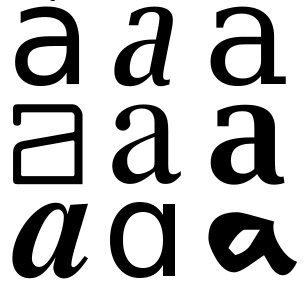
\includegraphics[scale=0.5]{images/nn.png}

The neural network will then use the examples to automatically determine some rules for reading the handwritten letters. Of course this example doenst have a lot of different types of the letter “A” so if we want to let the neural network become better at reading the handwritten letter “A” we would have to give it an example with many more examples of the letter. It would improve the accuracy, therefore it is better to provide the neural network with a thorough example.


\textit{"...a computing system made up of a number of simple, highly interconnected processing elements, which process information by their dynamic state response to external inputs.”}
A neural network consists of neurons which can send signals to each other. Each neuron processes its input signals and determines if the signal needs to be sent further. 
A neural network is not being fed with rules but instead examples that it can make rules from. With that a neural network is able to learn new skills, which is something that the traditionel computer cant do.

There are several types of neural networks and are being distinguished by their type (feedforward or feedback), their structure, and the learning algorithm that they use.
Feedforward neural networks will only allow the neurons to connect between two different layers. The feedback type of neural network will have a connection between neurons which are of the same layer but also between the different layers.

\subsection{Test}


\subsection{Discussion}

\subsection{Conclusion}